\begin{frame} 
\frametitle{Code: Gegeben}

\only<2->{
\texttt{generate\_BBsignal}   
\only<3->{ : musste implementiert werden  } 

\smallbreak
\texttt{measure\_H} 
\only<4->{ : bereits gegeben in Python  }

\smallbreak
\texttt{compute\_Uquest}  
\only<5->{ : bereits gegeben in Matlab und Python  }

\smallbreak
\texttt{compute\_Uin} 
\only<6->{ : bereits gegeben in Matlab }

\smallbreak
\texttt{measure\_Uout} 
\only<7->{ : writeAWG.py und writeDSO.py waren gegeben  }

\smallbreak
\texttt{compute\_a} 
\only<8->{ : geben in Matlab }

\smallbreak
\texttt{compute\_K} 
\only<9->{ : bereits gegeben in Matlab und Python   }

\only<10->
{
	\begin{textblock}{20}(63,55)
    	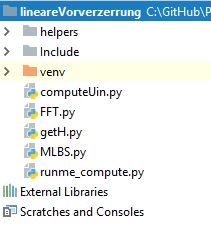
\includegraphics[scale=0.5 ]{slides/Gegeben/lineareFiles.JPG} 
	\end{textblock}	
	\begin{textblock}{20}(93,55)
    	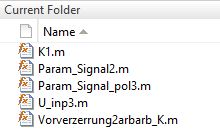
\includegraphics[scale=0.5 ]{slides/Gegeben/matlabFiles.JPG} 
	\end{textblock}	
}

}
\end{frame}


\begin{frame}
\frametitle{Code: Vorgehensweise}

\only<2->{
\begin{itemize}
	\only<1->{\item Refactoring / Anpassung der Matlab-Funktionen an unser Design}
	\only<3->{\item Portierung der Matlab-Funktionen nach Python}
	\only<4->{\item Überprüfung der portierten Funktionen mithilfe von \textbf{TDD}}
	\only<5->	
	{
		\begin{itemize}
			\item  Momentan jeweils 10 korrespondierende \textbf{Unit Tests} in Matlab und Python
		\end{itemize}
	}
	\only<6->{\item Maximale Vorbereitung der Funktionen ohne die Geräte dank \textbf{TDD}}
	\only<7->
	{
		\begin{itemize}
			\item  Nur fürs Testen von \texttt{measure\_Uout} sind Geräte notwendig
		\end{itemize}
	}		
\end{itemize}
}
 

\end{frame}
